% Options for packages loaded elsewhere
\PassOptionsToPackage{unicode}{hyperref}
\PassOptionsToPackage{hyphens}{url}
%
\documentclass[
]{article}
\title{HW4}
\author{Nikhil Gopal}
\date{11/6/2021}

\usepackage{amsmath,amssymb}
\usepackage{lmodern}
\usepackage{iftex}
\ifPDFTeX
  \usepackage[T1]{fontenc}
  \usepackage[utf8]{inputenc}
  \usepackage{textcomp} % provide euro and other symbols
\else % if luatex or xetex
  \usepackage{unicode-math}
  \defaultfontfeatures{Scale=MatchLowercase}
  \defaultfontfeatures[\rmfamily]{Ligatures=TeX,Scale=1}
\fi
% Use upquote if available, for straight quotes in verbatim environments
\IfFileExists{upquote.sty}{\usepackage{upquote}}{}
\IfFileExists{microtype.sty}{% use microtype if available
  \usepackage[]{microtype}
  \UseMicrotypeSet[protrusion]{basicmath} % disable protrusion for tt fonts
}{}
\makeatletter
\@ifundefined{KOMAClassName}{% if non-KOMA class
  \IfFileExists{parskip.sty}{%
    \usepackage{parskip}
  }{% else
    \setlength{\parindent}{0pt}
    \setlength{\parskip}{6pt plus 2pt minus 1pt}}
}{% if KOMA class
  \KOMAoptions{parskip=half}}
\makeatother
\usepackage{xcolor}
\IfFileExists{xurl.sty}{\usepackage{xurl}}{} % add URL line breaks if available
\IfFileExists{bookmark.sty}{\usepackage{bookmark}}{\usepackage{hyperref}}
\hypersetup{
  pdftitle={HW4},
  pdfauthor={Nikhil Gopal},
  hidelinks,
  pdfcreator={LaTeX via pandoc}}
\urlstyle{same} % disable monospaced font for URLs
\usepackage[margin=1in]{geometry}
\usepackage{color}
\usepackage{fancyvrb}
\newcommand{\VerbBar}{|}
\newcommand{\VERB}{\Verb[commandchars=\\\{\}]}
\DefineVerbatimEnvironment{Highlighting}{Verbatim}{commandchars=\\\{\}}
% Add ',fontsize=\small' for more characters per line
\usepackage{framed}
\definecolor{shadecolor}{RGB}{248,248,248}
\newenvironment{Shaded}{\begin{snugshade}}{\end{snugshade}}
\newcommand{\AlertTok}[1]{\textcolor[rgb]{0.94,0.16,0.16}{#1}}
\newcommand{\AnnotationTok}[1]{\textcolor[rgb]{0.56,0.35,0.01}{\textbf{\textit{#1}}}}
\newcommand{\AttributeTok}[1]{\textcolor[rgb]{0.77,0.63,0.00}{#1}}
\newcommand{\BaseNTok}[1]{\textcolor[rgb]{0.00,0.00,0.81}{#1}}
\newcommand{\BuiltInTok}[1]{#1}
\newcommand{\CharTok}[1]{\textcolor[rgb]{0.31,0.60,0.02}{#1}}
\newcommand{\CommentTok}[1]{\textcolor[rgb]{0.56,0.35,0.01}{\textit{#1}}}
\newcommand{\CommentVarTok}[1]{\textcolor[rgb]{0.56,0.35,0.01}{\textbf{\textit{#1}}}}
\newcommand{\ConstantTok}[1]{\textcolor[rgb]{0.00,0.00,0.00}{#1}}
\newcommand{\ControlFlowTok}[1]{\textcolor[rgb]{0.13,0.29,0.53}{\textbf{#1}}}
\newcommand{\DataTypeTok}[1]{\textcolor[rgb]{0.13,0.29,0.53}{#1}}
\newcommand{\DecValTok}[1]{\textcolor[rgb]{0.00,0.00,0.81}{#1}}
\newcommand{\DocumentationTok}[1]{\textcolor[rgb]{0.56,0.35,0.01}{\textbf{\textit{#1}}}}
\newcommand{\ErrorTok}[1]{\textcolor[rgb]{0.64,0.00,0.00}{\textbf{#1}}}
\newcommand{\ExtensionTok}[1]{#1}
\newcommand{\FloatTok}[1]{\textcolor[rgb]{0.00,0.00,0.81}{#1}}
\newcommand{\FunctionTok}[1]{\textcolor[rgb]{0.00,0.00,0.00}{#1}}
\newcommand{\ImportTok}[1]{#1}
\newcommand{\InformationTok}[1]{\textcolor[rgb]{0.56,0.35,0.01}{\textbf{\textit{#1}}}}
\newcommand{\KeywordTok}[1]{\textcolor[rgb]{0.13,0.29,0.53}{\textbf{#1}}}
\newcommand{\NormalTok}[1]{#1}
\newcommand{\OperatorTok}[1]{\textcolor[rgb]{0.81,0.36,0.00}{\textbf{#1}}}
\newcommand{\OtherTok}[1]{\textcolor[rgb]{0.56,0.35,0.01}{#1}}
\newcommand{\PreprocessorTok}[1]{\textcolor[rgb]{0.56,0.35,0.01}{\textit{#1}}}
\newcommand{\RegionMarkerTok}[1]{#1}
\newcommand{\SpecialCharTok}[1]{\textcolor[rgb]{0.00,0.00,0.00}{#1}}
\newcommand{\SpecialStringTok}[1]{\textcolor[rgb]{0.31,0.60,0.02}{#1}}
\newcommand{\StringTok}[1]{\textcolor[rgb]{0.31,0.60,0.02}{#1}}
\newcommand{\VariableTok}[1]{\textcolor[rgb]{0.00,0.00,0.00}{#1}}
\newcommand{\VerbatimStringTok}[1]{\textcolor[rgb]{0.31,0.60,0.02}{#1}}
\newcommand{\WarningTok}[1]{\textcolor[rgb]{0.56,0.35,0.01}{\textbf{\textit{#1}}}}
\usepackage{graphicx}
\makeatletter
\def\maxwidth{\ifdim\Gin@nat@width>\linewidth\linewidth\else\Gin@nat@width\fi}
\def\maxheight{\ifdim\Gin@nat@height>\textheight\textheight\else\Gin@nat@height\fi}
\makeatother
% Scale images if necessary, so that they will not overflow the page
% margins by default, and it is still possible to overwrite the defaults
% using explicit options in \includegraphics[width, height, ...]{}
\setkeys{Gin}{width=\maxwidth,height=\maxheight,keepaspectratio}
% Set default figure placement to htbp
\makeatletter
\def\fps@figure{htbp}
\makeatother
\setlength{\emergencystretch}{3em} % prevent overfull lines
\providecommand{\tightlist}{%
  \setlength{\itemsep}{0pt}\setlength{\parskip}{0pt}}
\setcounter{secnumdepth}{-\maxdimen} % remove section numbering
\ifLuaTeX
  \usepackage{selnolig}  % disable illegal ligatures
\fi

\begin{document}
\maketitle

\textbf{1}

\begin{Shaded}
\begin{Highlighting}[]
\FunctionTok{library}\NormalTok{(datasets) }\CommentTok{\# Load iris data}
\FunctionTok{library}\NormalTok{(ggplot2)}
\FunctionTok{library}\NormalTok{(nnet) }\CommentTok{\# For multinomial logistic regression}
\FunctionTok{library}\NormalTok{(naivebayes)}
\end{Highlighting}
\end{Shaded}

\begin{verbatim}
## naivebayes 0.9.7 loaded
\end{verbatim}

\begin{Shaded}
\begin{Highlighting}[]
\FunctionTok{library}\NormalTok{(adabag) }\CommentTok{\# For AdaBoost}
\end{Highlighting}
\end{Shaded}

\begin{verbatim}
## Loading required package: rpart
\end{verbatim}

\begin{verbatim}
## Loading required package: caret
\end{verbatim}

\begin{verbatim}
## Loading required package: lattice
\end{verbatim}

\begin{verbatim}
## Loading required package: foreach
\end{verbatim}

\begin{verbatim}
## Loading required package: doParallel
\end{verbatim}

\begin{verbatim}
## Loading required package: iterators
\end{verbatim}

\begin{verbatim}
## Loading required package: parallel
\end{verbatim}

\begin{Shaded}
\begin{Highlighting}[]
\FunctionTok{library}\NormalTok{(rpart) }\CommentTok{\# For AdaBoost}
\FunctionTok{library}\NormalTok{(tidyverse)}
\end{Highlighting}
\end{Shaded}

\begin{verbatim}
## -- Attaching packages --------------------------------------- tidyverse 1.3.1 --
\end{verbatim}

\begin{verbatim}
## v tibble  3.1.5     v dplyr   1.0.7
## v tidyr   1.1.4     v stringr 1.4.0
## v readr   2.0.2     v forcats 0.5.1
## v purrr   0.3.4
\end{verbatim}

\begin{verbatim}
## -- Conflicts ------------------------------------------ tidyverse_conflicts() --
## x purrr::accumulate() masks foreach::accumulate()
## x dplyr::filter()     masks stats::filter()
## x dplyr::lag()        masks stats::lag()
## x purrr::lift()       masks caret::lift()
## x purrr::when()       masks foreach::when()
\end{verbatim}

\begin{Shaded}
\begin{Highlighting}[]
\FunctionTok{library}\NormalTok{(ggpubr)}
\FunctionTok{library}\NormalTok{(caret)}
\FunctionTok{library}\NormalTok{(lmtest)}
\end{Highlighting}
\end{Shaded}

\begin{verbatim}
## Loading required package: zoo
\end{verbatim}

\begin{verbatim}
## 
## Attaching package: 'zoo'
\end{verbatim}

\begin{verbatim}
## The following objects are masked from 'package:base':
## 
##     as.Date, as.Date.numeric
\end{verbatim}

1a Boxplots, Correlation Matrix, Scatter Plots of Features Pairs:

\begin{Shaded}
\begin{Highlighting}[]
\NormalTok{data }\OtherTok{\textless{}{-}}\NormalTok{ iris}

\CommentTok{\#Boxplots}
\FunctionTok{boxplot}\NormalTok{(data}\SpecialCharTok{$}\NormalTok{Sepal.Length, }\AttributeTok{main =} \StringTok{"Sepal Length"}\NormalTok{)}
\end{Highlighting}
\end{Shaded}

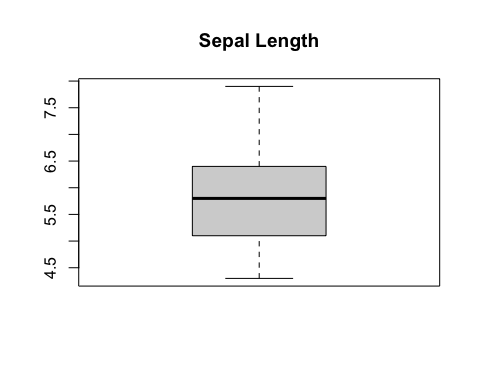
\includegraphics{HW4_files/figure-latex/unnamed-chunk-2-1.pdf}

\begin{Shaded}
\begin{Highlighting}[]
\FunctionTok{boxplot}\NormalTok{(data}\SpecialCharTok{$}\NormalTok{Sepal.Width, }\AttributeTok{main =} \StringTok{"Sepal Width"}\NormalTok{)}
\end{Highlighting}
\end{Shaded}

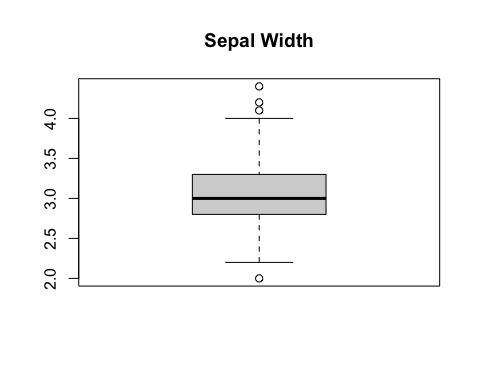
\includegraphics{HW4_files/figure-latex/unnamed-chunk-2-2.pdf}

\begin{Shaded}
\begin{Highlighting}[]
\FunctionTok{boxplot}\NormalTok{(data}\SpecialCharTok{$}\NormalTok{Petal.Length, }\AttributeTok{main =} \StringTok{"Petal Length"}\NormalTok{)}
\end{Highlighting}
\end{Shaded}

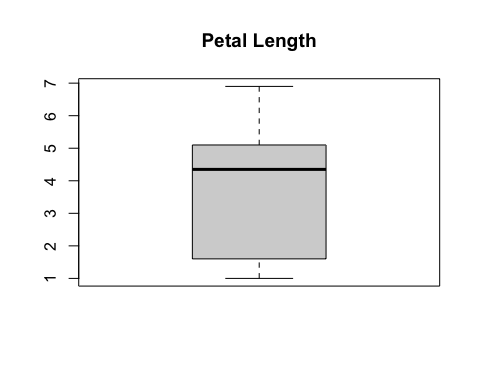
\includegraphics{HW4_files/figure-latex/unnamed-chunk-2-3.pdf}

\begin{Shaded}
\begin{Highlighting}[]
\FunctionTok{boxplot}\NormalTok{(data}\SpecialCharTok{$}\NormalTok{Petal.Width, }\AttributeTok{main =} \StringTok{"Petal Width"}\NormalTok{)}
\end{Highlighting}
\end{Shaded}

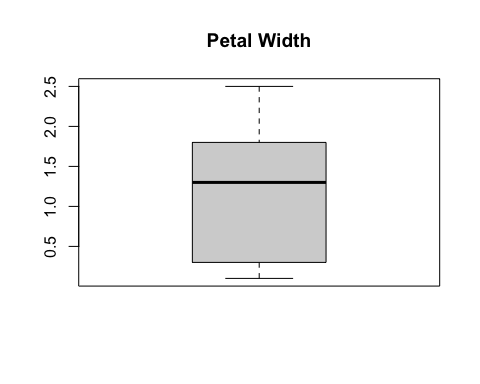
\includegraphics{HW4_files/figure-latex/unnamed-chunk-2-4.pdf}

\begin{Shaded}
\begin{Highlighting}[]
\CommentTok{\#boxplot(data$Species)}

\CommentTok{\#Correlation Matrix}
\FunctionTok{cor}\NormalTok{(data[}\DecValTok{1}\SpecialCharTok{:}\DecValTok{4}\NormalTok{])}
\end{Highlighting}
\end{Shaded}

\begin{verbatim}
##              Sepal.Length Sepal.Width Petal.Length Petal.Width
## Sepal.Length    1.0000000  -0.1175698    0.8717538   0.8179411
## Sepal.Width    -0.1175698   1.0000000   -0.4284401  -0.3661259
## Petal.Length    0.8717538  -0.4284401    1.0000000   0.9628654
## Petal.Width     0.8179411  -0.3661259    0.9628654   1.0000000
\end{verbatim}

\begin{Shaded}
\begin{Highlighting}[]
\CommentTok{\#scatterplots}
\FunctionTok{ggplot}\NormalTok{(iris, }\FunctionTok{aes}\NormalTok{(}\AttributeTok{x=}\NormalTok{Sepal.Length, }\AttributeTok{y=}\NormalTok{Sepal.Width, }\AttributeTok{color =}\NormalTok{ Species)) }\SpecialCharTok{+} \FunctionTok{geom\_point}\NormalTok{()}
\end{Highlighting}
\end{Shaded}

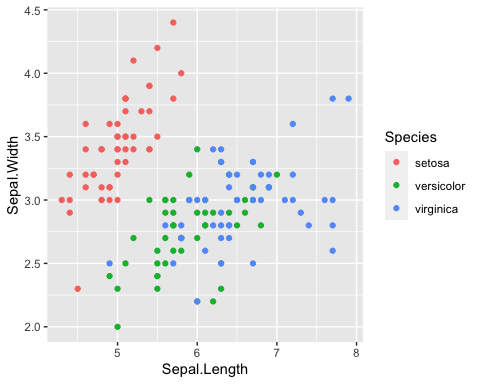
\includegraphics{HW4_files/figure-latex/unnamed-chunk-2-5.pdf}

\begin{Shaded}
\begin{Highlighting}[]
\FunctionTok{ggplot}\NormalTok{(iris, }\FunctionTok{aes}\NormalTok{(}\AttributeTok{x=}\NormalTok{Sepal.Length, }\AttributeTok{y=}\NormalTok{Petal.Length, }\AttributeTok{color =}\NormalTok{ Species)) }\SpecialCharTok{+} \FunctionTok{geom\_point}\NormalTok{()}
\end{Highlighting}
\end{Shaded}

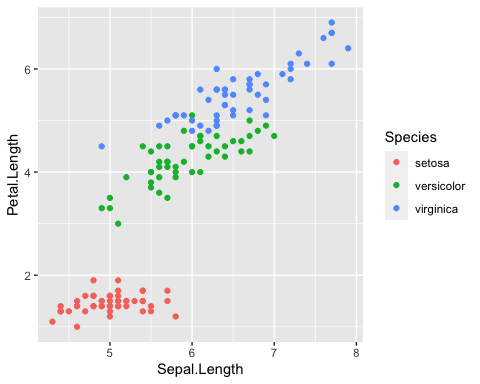
\includegraphics{HW4_files/figure-latex/unnamed-chunk-2-6.pdf}

\begin{Shaded}
\begin{Highlighting}[]
\FunctionTok{ggplot}\NormalTok{(iris, }\FunctionTok{aes}\NormalTok{(}\AttributeTok{x=}\NormalTok{Sepal.Length, }\AttributeTok{y=}\NormalTok{Petal.Width, }\AttributeTok{color =}\NormalTok{ Species)) }\SpecialCharTok{+} \FunctionTok{geom\_point}\NormalTok{()}
\end{Highlighting}
\end{Shaded}

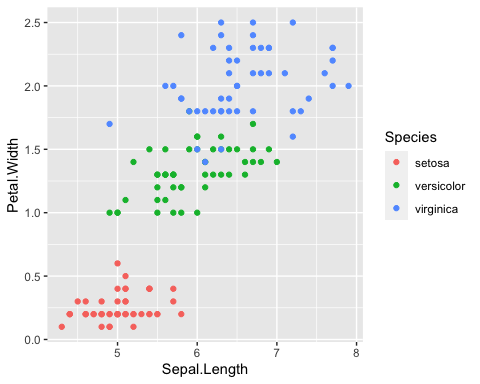
\includegraphics{HW4_files/figure-latex/unnamed-chunk-2-7.pdf}

\begin{Shaded}
\begin{Highlighting}[]
\FunctionTok{ggplot}\NormalTok{(iris, }\FunctionTok{aes}\NormalTok{(}\AttributeTok{x=}\NormalTok{Sepal.Width, }\AttributeTok{y=}\NormalTok{Petal.Length, }\AttributeTok{color =}\NormalTok{ Species)) }\SpecialCharTok{+} \FunctionTok{geom\_point}\NormalTok{()}
\end{Highlighting}
\end{Shaded}

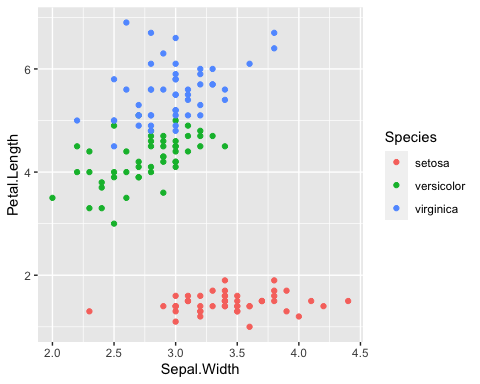
\includegraphics{HW4_files/figure-latex/unnamed-chunk-2-8.pdf}

\begin{Shaded}
\begin{Highlighting}[]
\FunctionTok{ggplot}\NormalTok{(iris, }\FunctionTok{aes}\NormalTok{(}\AttributeTok{x=}\NormalTok{Sepal.Width, }\AttributeTok{y=}\NormalTok{Petal.Width, }\AttributeTok{color =}\NormalTok{ Species)) }\SpecialCharTok{+} \FunctionTok{geom\_point}\NormalTok{()}
\end{Highlighting}
\end{Shaded}

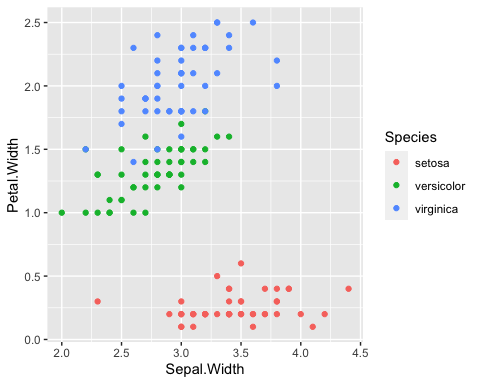
\includegraphics{HW4_files/figure-latex/unnamed-chunk-2-9.pdf}

\begin{Shaded}
\begin{Highlighting}[]
\FunctionTok{ggplot}\NormalTok{(iris, }\FunctionTok{aes}\NormalTok{(}\AttributeTok{x=}\NormalTok{Petal.Length, }\AttributeTok{y=}\NormalTok{Petal.Width, }\AttributeTok{color =}\NormalTok{ Species)) }\SpecialCharTok{+} \FunctionTok{geom\_point}\NormalTok{()}
\end{Highlighting}
\end{Shaded}

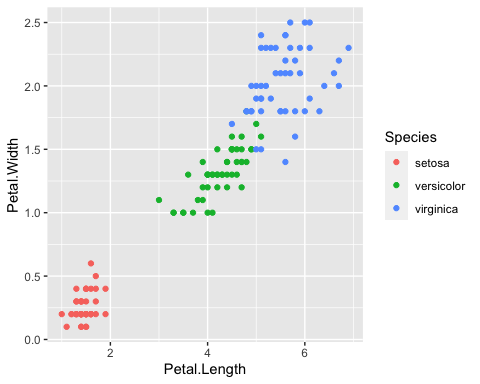
\includegraphics{HW4_files/figure-latex/unnamed-chunk-2-10.pdf}

1b:

Use X1, X2, X3 to fit the multinomial logistic regression, the Naive
Bayes classifier, and the AdaBoost with 30 Decision Tree classifiers
with maximum depth 3. Plot the decision surfaces of the 3 classifiers on
(X1, X2) and (X1, X3) respectively.

\begin{Shaded}
\begin{Highlighting}[]
\CommentTok{\# Fit a multinomial logistic regression}
\NormalTok{multinom\_model }\OtherTok{\textless{}{-}} \FunctionTok{multinom}\NormalTok{(Species }\SpecialCharTok{\textasciitilde{}}\NormalTok{ Sepal.Length }\SpecialCharTok{+}\NormalTok{ Sepal.Width }\SpecialCharTok{+}\NormalTok{ Petal.Length, }\AttributeTok{data=}\NormalTok{iris)}
\end{Highlighting}
\end{Shaded}

\begin{verbatim}
## # weights:  15 (8 variable)
## initial  value 164.791843 
## iter  10 value 21.394999
## iter  20 value 13.010468
## iter  30 value 11.932227
## iter  40 value 11.899523
## iter  50 value 11.886536
## final  value 11.886441 
## converged
\end{verbatim}

\begin{Shaded}
\begin{Highlighting}[]
\CommentTok{\# Generate grid points for plotting decision surfaces}
\NormalTok{r }\OtherTok{\textless{}{-}} \FunctionTok{sapply}\NormalTok{(iris[, }\FunctionTok{c}\NormalTok{(}\DecValTok{1}\NormalTok{,}\DecValTok{2}\NormalTok{,}\DecValTok{3}\NormalTok{)], range, }\AttributeTok{na.rm =} \ConstantTok{TRUE}\NormalTok{)}
\NormalTok{x1s }\OtherTok{\textless{}{-}} \FunctionTok{seq}\NormalTok{(r[}\DecValTok{1}\NormalTok{,}\DecValTok{1}\NormalTok{], r[}\DecValTok{2}\NormalTok{,}\DecValTok{1}\NormalTok{], }\AttributeTok{length.out =} \DecValTok{500}\NormalTok{)}
\NormalTok{x3s }\OtherTok{\textless{}{-}} \FunctionTok{seq}\NormalTok{(r[}\DecValTok{1}\NormalTok{,}\DecValTok{2}\NormalTok{], r[}\DecValTok{2}\NormalTok{,}\DecValTok{2}\NormalTok{], }\AttributeTok{length.out =} \DecValTok{500}\NormalTok{)}
\NormalTok{x4s }\OtherTok{\textless{}{-}} \FunctionTok{seq}\NormalTok{(r[}\DecValTok{1}\NormalTok{,}\DecValTok{3}\NormalTok{], r[}\DecValTok{2}\NormalTok{,}\DecValTok{3}\NormalTok{], }\AttributeTok{length.out =} \DecValTok{500}\NormalTok{)}
\NormalTok{grid }\OtherTok{\textless{}{-}} \FunctionTok{cbind}\NormalTok{(}\FunctionTok{rep}\NormalTok{(x1s, }\AttributeTok{each=}\DecValTok{500}\NormalTok{), }\FunctionTok{rep}\NormalTok{(x3s, }\AttributeTok{time =} \DecValTok{500}\NormalTok{), }\FunctionTok{rep}\NormalTok{(x4s, }\AttributeTok{time =} \DecValTok{500}\NormalTok{))}
\FunctionTok{colnames}\NormalTok{(grid) }\OtherTok{\textless{}{-}} \FunctionTok{colnames}\NormalTok{(r)}
\NormalTok{grid }\OtherTok{\textless{}{-}} \FunctionTok{as.data.frame}\NormalTok{(grid)}

\CommentTok{\# Predictions from the generated grid points}
\NormalTok{multinom\_pred }\OtherTok{\textless{}{-}} \FunctionTok{predict}\NormalTok{(multinom\_model, }\AttributeTok{newdata=}\NormalTok{grid, }\AttributeTok{type=}\StringTok{"class"}\NormalTok{)}


\CommentTok{\# For Naive Bayes, simply replace the lines for model fitting and prediction with:}
\NormalTok{nb\_model }\OtherTok{\textless{}{-}} \FunctionTok{naive\_bayes}\NormalTok{(Species }\SpecialCharTok{\textasciitilde{}}\NormalTok{ Sepal.Length }\SpecialCharTok{+}\NormalTok{ Sepal.Width }\SpecialCharTok{+}\NormalTok{ Petal.Length, }\AttributeTok{data =}\NormalTok{ iris)}
\NormalTok{nb\_pred }\OtherTok{\textless{}{-}} \FunctionTok{predict}\NormalTok{(nb\_model, grid, }\AttributeTok{type =} \StringTok{"class"}\NormalTok{)}

\CommentTok{\# Plot decision surfaces for (X1, X2)}
\NormalTok{mult\_ds1 }\OtherTok{\textless{}{-}} \FunctionTok{ggplot}\NormalTok{() }\SpecialCharTok{+} 
  \FunctionTok{geom\_point}\NormalTok{(}\AttributeTok{data =}\NormalTok{ iris, }\FunctionTok{aes}\NormalTok{(}\AttributeTok{x=}\NormalTok{Sepal.Length, }\AttributeTok{y=}\NormalTok{Sepal.Width, }\AttributeTok{color =}\NormalTok{ Species), }\AttributeTok{size =} \DecValTok{2}\NormalTok{, }\AttributeTok{show.legend =}\NormalTok{ F) }\SpecialCharTok{+}
  \FunctionTok{geom\_raster}\NormalTok{(}\AttributeTok{alpha=}\FloatTok{0.1}\NormalTok{, }\FunctionTok{aes}\NormalTok{(}\AttributeTok{x =}\NormalTok{ grid[, }\DecValTok{1}\NormalTok{],}\AttributeTok{y =}\NormalTok{ grid[, }\DecValTok{2}\NormalTok{], }\AttributeTok{fill=}\NormalTok{multinom\_pred), }\AttributeTok{show.legend =}\NormalTok{ F) }\SpecialCharTok{+}
  \FunctionTok{theme\_bw}\NormalTok{()}

\NormalTok{nb\_ds1 }\OtherTok{\textless{}{-}} \FunctionTok{ggplot}\NormalTok{() }\SpecialCharTok{+} 
  \FunctionTok{geom\_point}\NormalTok{(}\AttributeTok{data =}\NormalTok{ iris, }\FunctionTok{aes}\NormalTok{(}\AttributeTok{x=}\NormalTok{Sepal.Length, }\AttributeTok{y=}\NormalTok{Sepal.Width, }\AttributeTok{color =}\NormalTok{ Species), }\AttributeTok{size =} \DecValTok{2}\NormalTok{, }\AttributeTok{show.legend =}\NormalTok{ F) }\SpecialCharTok{+}
  \FunctionTok{geom\_raster}\NormalTok{(}\AttributeTok{alpha=}\FloatTok{0.1}\NormalTok{, }\FunctionTok{aes}\NormalTok{(}\AttributeTok{x =}\NormalTok{ grid[, }\DecValTok{1}\NormalTok{],}\AttributeTok{y =}\NormalTok{ grid[, }\DecValTok{2}\NormalTok{], }\AttributeTok{fill=}\NormalTok{nb\_pred), }\AttributeTok{show.legend =}\NormalTok{ F) }\SpecialCharTok{+}
  \FunctionTok{theme\_bw}\NormalTok{()}

\NormalTok{boost\_ds1 }\OtherTok{\textless{}{-}} \FunctionTok{ggplot}\NormalTok{() }\SpecialCharTok{+} 
  \FunctionTok{geom\_point}\NormalTok{(}\AttributeTok{data =}\NormalTok{ iris, }\FunctionTok{aes}\NormalTok{(}\AttributeTok{x=}\NormalTok{Sepal.Length, }\AttributeTok{y=}\NormalTok{Sepal.Width, }\AttributeTok{color =}\NormalTok{ Species), }\AttributeTok{size =} \DecValTok{2}\NormalTok{, }\AttributeTok{show.legend =}\NormalTok{ F) }\SpecialCharTok{+}
  \FunctionTok{geom\_raster}\NormalTok{(}\AttributeTok{alpha=}\FloatTok{0.1}\NormalTok{, }\FunctionTok{aes}\NormalTok{(}\AttributeTok{x =}\NormalTok{ grid[, }\DecValTok{1}\NormalTok{],}\AttributeTok{y =}\NormalTok{ grid[, }\DecValTok{2}\NormalTok{], }\AttributeTok{fill=}\NormalTok{boost\_pred), }\AttributeTok{show.legend =}\NormalTok{ F) }\SpecialCharTok{+}
  \FunctionTok{theme\_bw}\NormalTok{()}



\CommentTok{\# For AdaBoost:}
\NormalTok{boost\_model }\OtherTok{\textless{}{-}} \FunctionTok{boosting}\NormalTok{(Species }\SpecialCharTok{\textasciitilde{}}\NormalTok{ Sepal.Length }\SpecialCharTok{+}\NormalTok{ Sepal.Width }\SpecialCharTok{+}\NormalTok{ Petal.Length,}
\AttributeTok{data =}\NormalTok{ iris, }\AttributeTok{mfinal =} \DecValTok{30}\NormalTok{, }\AttributeTok{control =} \FunctionTok{rpart.control}\NormalTok{(}\AttributeTok{maxdepth =} \DecValTok{3}\NormalTok{))}
\NormalTok{boost\_pred }\OtherTok{\textless{}{-}} \FunctionTok{predict}\NormalTok{(boost\_model, grid, }\AttributeTok{type =} \StringTok{"class"}\NormalTok{)}\SpecialCharTok{$}\NormalTok{class}


\FunctionTok{ggarrange}\NormalTok{(mult\_ds1, nb\_ds1, boost\_ds1, }\AttributeTok{ncol =} \DecValTok{2}\NormalTok{, }\AttributeTok{nrow =} \DecValTok{2}\NormalTok{)}
\end{Highlighting}
\end{Shaded}

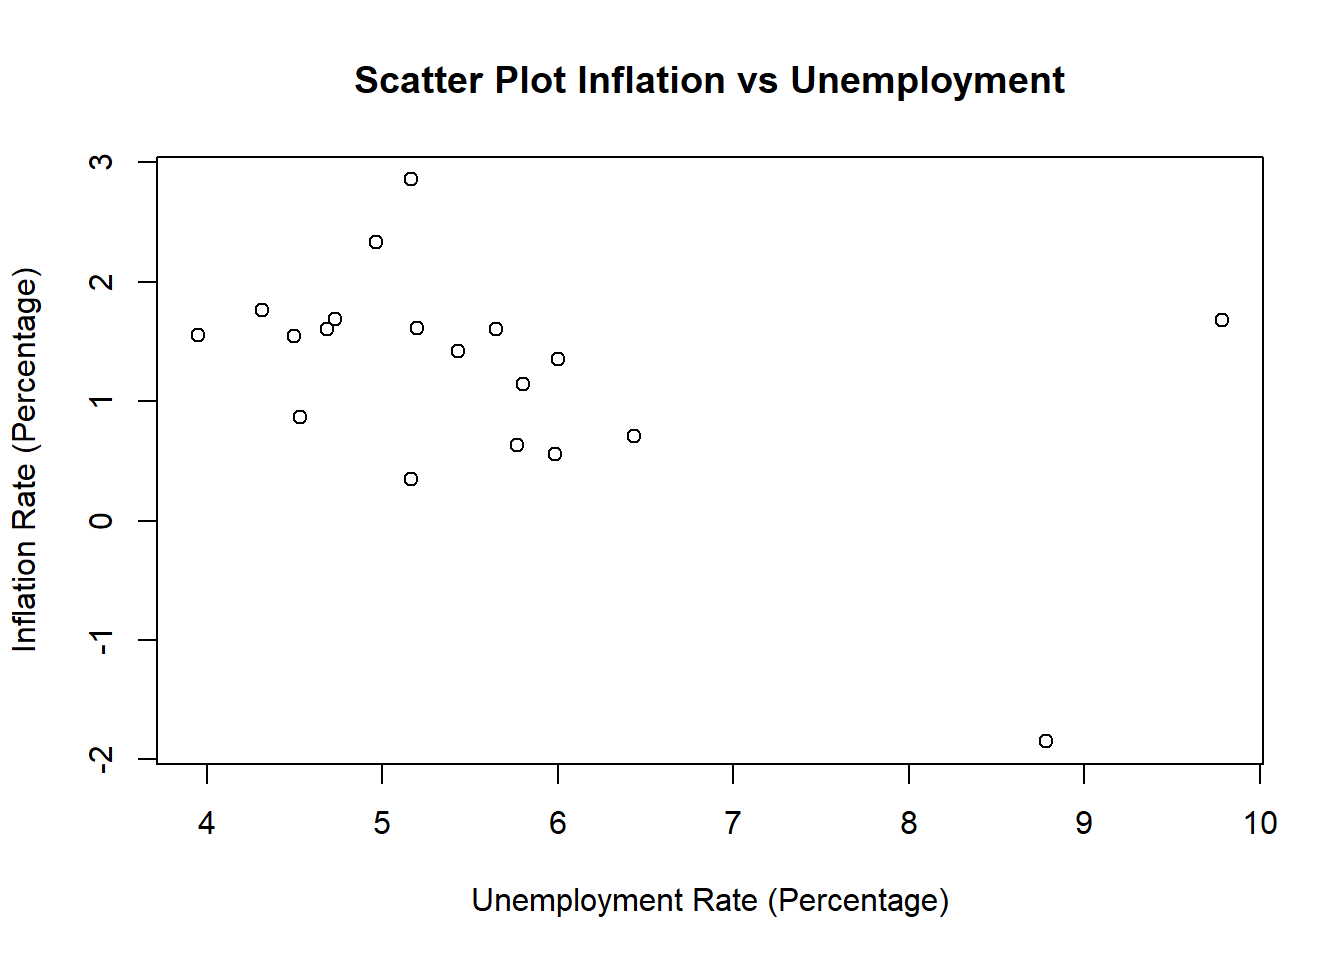
\includegraphics{HW4_files/figure-latex/unnamed-chunk-3-1.pdf}
\textbf{1c:}

Based on the decision surfaces, compare and summarize the advantage and
disadvantage of each classifier.

\textbf{2a:}

Creating correlated errors through time. Please write a function that
takes in an integer, n ≥1, then produces ``errors'' that are generated
in the following way:

\begin{Shaded}
\begin{Highlighting}[]
\NormalTok{generate\_errors }\OtherTok{\textless{}{-}} \ControlFlowTok{function}\NormalTok{(n)\{}
\NormalTok{  errors }\OtherTok{\textless{}{-}} \FunctionTok{c}\NormalTok{()}
  \ControlFlowTok{for}\NormalTok{ (i }\ControlFlowTok{in} \DecValTok{1}\SpecialCharTok{:}\NormalTok{n) \{}
    \ControlFlowTok{if}\NormalTok{(i }\SpecialCharTok{==} \DecValTok{1}\NormalTok{)\{}
\NormalTok{      errors }\OtherTok{\textless{}{-}} \FunctionTok{c}\NormalTok{(errors, }\FunctionTok{rnorm}\NormalTok{(}\DecValTok{1}\NormalTok{, }\DecValTok{0}\NormalTok{, }\DecValTok{1}\NormalTok{))}
\NormalTok{    \}}\ControlFlowTok{else}\NormalTok{\{}
\NormalTok{      errors }\OtherTok{\textless{}{-}} \FunctionTok{c}\NormalTok{(errors, }\FunctionTok{rnorm}\NormalTok{(}\DecValTok{1}\NormalTok{, }\AttributeTok{mean =} \FunctionTok{last}\NormalTok{(errors), }\AttributeTok{sd =} \DecValTok{1}\NormalTok{))}
\NormalTok{    \}}
\NormalTok{  \}}
  \FunctionTok{return}\NormalTok{(errors)}
\NormalTok{\}}
\end{Highlighting}
\end{Shaded}

\textbf{2b}

\begin{Shaded}
\begin{Highlighting}[]
\CommentTok{\#generate values}
\NormalTok{corr1 }\OtherTok{\textless{}{-}} \FunctionTok{generate\_errors}\NormalTok{(}\DecValTok{500}\NormalTok{)}
\NormalTok{rep1 }\OtherTok{\textless{}{-}} \FunctionTok{rep}\NormalTok{(}\DecValTok{1}\NormalTok{, }\DecValTok{500}\NormalTok{)}
\NormalTok{corr2 }\OtherTok{\textless{}{-}} \FunctionTok{generate\_errors}\NormalTok{(}\DecValTok{500}\NormalTok{)}
\NormalTok{rep2 }\OtherTok{\textless{}{-}} \FunctionTok{rep}\NormalTok{(}\DecValTok{2}\NormalTok{, }\DecValTok{500}\NormalTok{)}
\NormalTok{corr3 }\OtherTok{\textless{}{-}} \FunctionTok{generate\_errors}\NormalTok{(}\DecValTok{500}\NormalTok{)}
\NormalTok{rep3 }\OtherTok{\textless{}{-}} \FunctionTok{rep}\NormalTok{(}\DecValTok{3}\NormalTok{, }\DecValTok{500}\NormalTok{)}
\NormalTok{corr4 }\OtherTok{\textless{}{-}} \FunctionTok{generate\_errors}\NormalTok{(}\DecValTok{500}\NormalTok{)}
\NormalTok{rep4 }\OtherTok{\textless{}{-}} \FunctionTok{rep}\NormalTok{(}\DecValTok{4}\NormalTok{, }\DecValTok{500}\NormalTok{)}
\NormalTok{corr5 }\OtherTok{\textless{}{-}} \FunctionTok{generate\_errors}\NormalTok{(}\DecValTok{500}\NormalTok{)}
\NormalTok{rep5 }\OtherTok{\textless{}{-}} \FunctionTok{rep}\NormalTok{(}\DecValTok{5}\NormalTok{, }\DecValTok{500}\NormalTok{)}

\CommentTok{\#create a df}
\NormalTok{df }\OtherTok{\textless{}{-}} \FunctionTok{data\_frame}\NormalTok{(corr1, rep1)}
\end{Highlighting}
\end{Shaded}

\begin{verbatim}
## Warning: `data_frame()` was deprecated in tibble 1.1.0.
## Please use `tibble()` instead.
## This warning is displayed once every 8 hours.
## Call `lifecycle::last_lifecycle_warnings()` to see where this warning was generated.
\end{verbatim}

\begin{Shaded}
\begin{Highlighting}[]
\NormalTok{df2 }\OtherTok{\textless{}{-}} \FunctionTok{data\_frame}\NormalTok{(corr2, rep2)}
\NormalTok{df3 }\OtherTok{\textless{}{-}} \FunctionTok{data\_frame}\NormalTok{(corr3, rep3)}
\NormalTok{df4 }\OtherTok{\textless{}{-}} \FunctionTok{data\_frame}\NormalTok{(corr4, rep4)}
\NormalTok{df5 }\OtherTok{\textless{}{-}} \FunctionTok{data\_frame}\NormalTok{(corr5, rep5)}
\FunctionTok{names}\NormalTok{(df) }\OtherTok{\textless{}{-}} \FunctionTok{c}\NormalTok{(}\StringTok{"cor"}\NormalTok{, }\StringTok{"trial"}\NormalTok{)}
\FunctionTok{names}\NormalTok{(df2) }\OtherTok{\textless{}{-}} \FunctionTok{c}\NormalTok{(}\StringTok{"cor"}\NormalTok{, }\StringTok{"trial"}\NormalTok{)}
\FunctionTok{names}\NormalTok{(df3) }\OtherTok{\textless{}{-}} \FunctionTok{c}\NormalTok{(}\StringTok{"cor"}\NormalTok{, }\StringTok{"trial"}\NormalTok{)}
\FunctionTok{names}\NormalTok{(df4) }\OtherTok{\textless{}{-}} \FunctionTok{c}\NormalTok{(}\StringTok{"cor"}\NormalTok{, }\StringTok{"trial"}\NormalTok{)}
\FunctionTok{names}\NormalTok{(df5) }\OtherTok{\textless{}{-}} \FunctionTok{c}\NormalTok{(}\StringTok{"cor"}\NormalTok{, }\StringTok{"trial"}\NormalTok{)}

\NormalTok{final\_df }\OtherTok{\textless{}{-}} \FunctionTok{rbind}\NormalTok{(df, df2, df3, df4, df5)}
\NormalTok{final\_df}\SpecialCharTok{$}\NormalTok{index }\OtherTok{\textless{}{-}} \FunctionTok{rep}\NormalTok{(}\DecValTok{1}\SpecialCharTok{:}\DecValTok{2500}\NormalTok{)}

\FunctionTok{library}\NormalTok{(RColorBrewer)}

\CommentTok{\#correlated errors plot}
\NormalTok{cor\_plot }\OtherTok{\textless{}{-}} \FunctionTok{ggplot}\NormalTok{(final\_df, }\FunctionTok{aes}\NormalTok{(}\AttributeTok{x=}\NormalTok{index, }\AttributeTok{y =}\NormalTok{ cor, }\AttributeTok{color =}\NormalTok{ trial)) }\SpecialCharTok{+} \FunctionTok{geom\_point}\NormalTok{()}\SpecialCharTok{+} \FunctionTok{scale\_fill\_brewer}\NormalTok{(}\AttributeTok{palette=}\StringTok{"Dark2"}\NormalTok{)}


\CommentTok{\#uncorrelated errors}
\NormalTok{uncorr1 }\OtherTok{\textless{}{-}} \FunctionTok{rnorm}\NormalTok{(}\DecValTok{500}\NormalTok{, }\DecValTok{0}\NormalTok{, }\DecValTok{1}\NormalTok{)}
\NormalTok{unrep1 }\OtherTok{\textless{}{-}} \FunctionTok{rep}\NormalTok{(}\DecValTok{1}\NormalTok{, }\DecValTok{500}\NormalTok{)}
\NormalTok{uncorr2 }\OtherTok{\textless{}{-}} \FunctionTok{rnorm}\NormalTok{(}\DecValTok{500}\NormalTok{, }\DecValTok{0}\NormalTok{, }\DecValTok{1}\NormalTok{)}
\NormalTok{unrep2 }\OtherTok{\textless{}{-}} \FunctionTok{rep}\NormalTok{(}\DecValTok{2}\NormalTok{, }\DecValTok{500}\NormalTok{)}
\NormalTok{uncorr3 }\OtherTok{\textless{}{-}} \FunctionTok{rnorm}\NormalTok{(}\DecValTok{500}\NormalTok{, }\DecValTok{0}\NormalTok{, }\DecValTok{1}\NormalTok{)}
\NormalTok{unrep3 }\OtherTok{\textless{}{-}} \FunctionTok{rep}\NormalTok{(}\DecValTok{3}\NormalTok{, }\DecValTok{500}\NormalTok{)}
\NormalTok{uncorr4 }\OtherTok{\textless{}{-}} \FunctionTok{rnorm}\NormalTok{(}\DecValTok{500}\NormalTok{, }\DecValTok{0}\NormalTok{, }\DecValTok{1}\NormalTok{)}
\NormalTok{unrep4 }\OtherTok{\textless{}{-}} \FunctionTok{rep}\NormalTok{(}\DecValTok{4}\NormalTok{, }\DecValTok{500}\NormalTok{)}
\NormalTok{uncorr5 }\OtherTok{\textless{}{-}} \FunctionTok{rnorm}\NormalTok{(}\DecValTok{500}\NormalTok{, }\DecValTok{0}\NormalTok{, }\DecValTok{1}\NormalTok{)}
\NormalTok{unrep5 }\OtherTok{\textless{}{-}} \FunctionTok{rep}\NormalTok{(}\DecValTok{5}\NormalTok{, }\DecValTok{500}\NormalTok{)}

\CommentTok{\#create df}
\NormalTok{df }\OtherTok{\textless{}{-}} \FunctionTok{data\_frame}\NormalTok{(uncorr1, unrep1)}
\NormalTok{df2 }\OtherTok{\textless{}{-}} \FunctionTok{data\_frame}\NormalTok{(uncorr2, unrep2)}
\NormalTok{df3 }\OtherTok{\textless{}{-}} \FunctionTok{data\_frame}\NormalTok{(uncorr3, unrep3)}
\NormalTok{df4 }\OtherTok{\textless{}{-}} \FunctionTok{data\_frame}\NormalTok{(uncorr4, unrep4)}
\NormalTok{df5 }\OtherTok{\textless{}{-}} \FunctionTok{data\_frame}\NormalTok{(uncorr5, unrep5)}
\FunctionTok{names}\NormalTok{(df) }\OtherTok{\textless{}{-}} \FunctionTok{c}\NormalTok{(}\StringTok{"cor"}\NormalTok{, }\StringTok{"trial"}\NormalTok{)}
\FunctionTok{names}\NormalTok{(df2) }\OtherTok{\textless{}{-}} \FunctionTok{c}\NormalTok{(}\StringTok{"cor"}\NormalTok{, }\StringTok{"trial"}\NormalTok{)}
\FunctionTok{names}\NormalTok{(df3) }\OtherTok{\textless{}{-}} \FunctionTok{c}\NormalTok{(}\StringTok{"cor"}\NormalTok{, }\StringTok{"trial"}\NormalTok{)}
\FunctionTok{names}\NormalTok{(df4) }\OtherTok{\textless{}{-}} \FunctionTok{c}\NormalTok{(}\StringTok{"cor"}\NormalTok{, }\StringTok{"trial"}\NormalTok{)}
\FunctionTok{names}\NormalTok{(df5) }\OtherTok{\textless{}{-}} \FunctionTok{c}\NormalTok{(}\StringTok{"cor"}\NormalTok{, }\StringTok{"trial"}\NormalTok{)}

\NormalTok{uncor\_df }\OtherTok{\textless{}{-}} \FunctionTok{rbind}\NormalTok{(df, df2, df3, df4, df5)}
\NormalTok{uncor\_df}\SpecialCharTok{$}\NormalTok{index }\OtherTok{\textless{}{-}} \FunctionTok{rep}\NormalTok{(}\DecValTok{1}\SpecialCharTok{:}\DecValTok{2500}\NormalTok{)}

\CommentTok{\#uncorrelated errors plot}
\NormalTok{uncor\_plot }\OtherTok{\textless{}{-}} \FunctionTok{ggplot}\NormalTok{(uncor\_df, }\FunctionTok{aes}\NormalTok{(}\AttributeTok{x=}\NormalTok{index, }\AttributeTok{y =}\NormalTok{ cor, }\AttributeTok{color =}\NormalTok{ trial)) }\SpecialCharTok{+} \FunctionTok{geom\_point}\NormalTok{()}\SpecialCharTok{+} \FunctionTok{scale\_fill\_brewer}\NormalTok{(}\AttributeTok{palette=}\StringTok{"Dark2"}\NormalTok{)}

\CommentTok{\#show graphs}
\NormalTok{cor\_plot}
\end{Highlighting}
\end{Shaded}

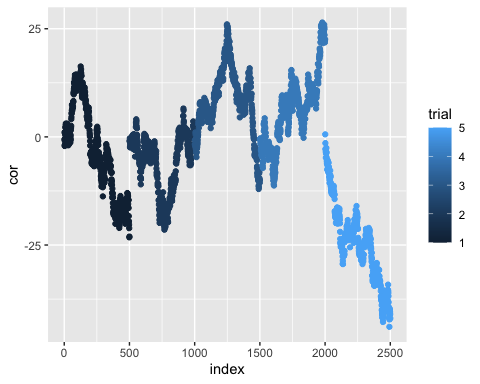
\includegraphics{HW4_files/figure-latex/unnamed-chunk-5-1.pdf}

\begin{Shaded}
\begin{Highlighting}[]
\NormalTok{uncor\_plot}
\end{Highlighting}
\end{Shaded}

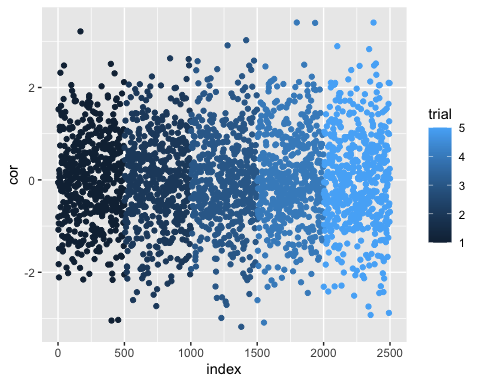
\includegraphics{HW4_files/figure-latex/unnamed-chunk-5-2.pdf}

\begin{Shaded}
\begin{Highlighting}[]
\NormalTok{rnoise }\OtherTok{\textless{}{-}} \ControlFlowTok{function}\NormalTok{(n) \{}
\NormalTok{  eps }\OtherTok{\textless{}{-}} \FunctionTok{vector}\NormalTok{(}\AttributeTok{length=}\NormalTok{n)}
\NormalTok{  eps[}\DecValTok{1}\NormalTok{] }\OtherTok{\textless{}{-}} \FunctionTok{rnorm}\NormalTok{(}\DecValTok{1}\NormalTok{, }\DecValTok{0}\NormalTok{, }\DecValTok{1}\NormalTok{)}
  \ControlFlowTok{for}\NormalTok{ (i }\ControlFlowTok{in} \DecValTok{2}\SpecialCharTok{:}\NormalTok{n)\{}
    \CommentTok{\#eps[i]\textless{}{-} rnorm(1, eps[i{-}1], 1)}
\NormalTok{    eps[i]}\OtherTok{\textless{}{-}}\NormalTok{ eps[i}\DecValTok{{-}1}\NormalTok{] }\SpecialCharTok{+} \FunctionTok{rnorm}\NormalTok{(}\DecValTok{1}\NormalTok{, }\DecValTok{0}\NormalTok{, }\DecValTok{1}\NormalTok{)}
\NormalTok{  \}}
  \FunctionTok{return}\NormalTok{(eps)}
\NormalTok{\}}


\NormalTok{num\_simulation }\OtherTok{\textless{}{-}} \DecValTok{5}
\NormalTok{correlated\_noise }\OtherTok{\textless{}{-}} \FunctionTok{replicate}\NormalTok{(num\_simulation, }\FunctionTok{rnoise}\NormalTok{(}\AttributeTok{n =} \DecValTok{500}\NormalTok{)) }
\NormalTok{independent\_noise }\OtherTok{\textless{}{-}} \FunctionTok{replicate}\NormalTok{(num\_simulation, }\FunctionTok{rnorm}\NormalTok{(}\AttributeTok{n =} \DecValTok{500}\NormalTok{))}

\FunctionTok{par}\NormalTok{(}\AttributeTok{mfrow=}\FunctionTok{c}\NormalTok{(}\DecValTok{1}\NormalTok{,}\DecValTok{2}\NormalTok{))}
\FunctionTok{matplot}\NormalTok{(correlated\_noise, }\AttributeTok{type=}\StringTok{"l"}\NormalTok{, }\AttributeTok{lty =} \DecValTok{1}\NormalTok{, }\AttributeTok{pch=}\DecValTok{19}\NormalTok{, }\AttributeTok{ylab=}\StringTok{"noise"}\NormalTok{, }\AttributeTok{xlab=}\StringTok{"n"}\NormalTok{, }\AttributeTok{main=}\StringTok{"Correlated"}\NormalTok{)}
\FunctionTok{matplot}\NormalTok{(independent\_noise, }\AttributeTok{type=}\StringTok{"l"}\NormalTok{, }\AttributeTok{lty =} \DecValTok{1}\NormalTok{, }\AttributeTok{pch=}\DecValTok{19}\NormalTok{, }\AttributeTok{ylab=}\StringTok{"noise"}\NormalTok{, }\AttributeTok{xlab=}\StringTok{"n"}\NormalTok{, }\AttributeTok{main=}\StringTok{"Independent"}\NormalTok{)}
\end{Highlighting}
\end{Shaded}

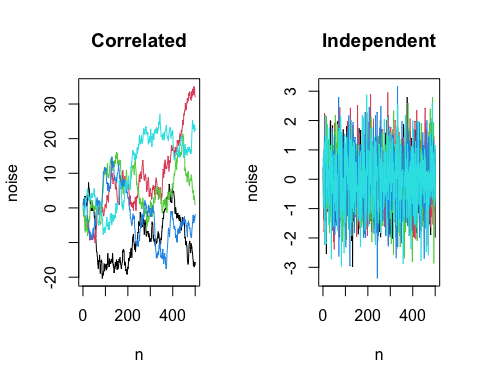
\includegraphics{HW4_files/figure-latex/unnamed-chunk-5-3.pdf}

\textbf{2c}

Comment on the difference. According to the plots you've created, please
answer the following:

Do both types of errors have mean 0 overall (1 sentence)? What could you
do to be more certain (1 sentence)?

The uncorrelated errors do have mean 0 overall, while the uncorrelated
errors definitely do not. We could calculate the average column values
in the dataframe and get this information quickly.

Uncorrelated:

\begin{Shaded}
\begin{Highlighting}[]
\FunctionTok{mean}\NormalTok{(uncor\_df}\SpecialCharTok{$}\NormalTok{cor)}
\end{Highlighting}
\end{Shaded}

\begin{verbatim}
## [1] -0.03478033
\end{verbatim}

Correlated:

\begin{Shaded}
\begin{Highlighting}[]
\FunctionTok{mean}\NormalTok{(final\_df}\SpecialCharTok{$}\NormalTok{cor)}
\end{Highlighting}
\end{Shaded}

\begin{verbatim}
## [1] 6.782941
\end{verbatim}

We see that the correlated has a mean of 1.39 (across each group) and
that the uncorrelated errors have a near zero mean of -0.001236516.

Which type of errors has a larger variance or are they comparable?

\begin{Shaded}
\begin{Highlighting}[]
\FunctionTok{var}\NormalTok{(final\_df}\SpecialCharTok{$}\NormalTok{cor)}
\end{Highlighting}
\end{Shaded}

\begin{verbatim}
## [1] 314.8409
\end{verbatim}

\begin{Shaded}
\begin{Highlighting}[]
\FunctionTok{var}\NormalTok{(uncor\_df}\SpecialCharTok{$}\NormalTok{cor)}
\end{Highlighting}
\end{Shaded}

\begin{verbatim}
## [1] 1.044982
\end{verbatim}

The correlated errors have a variance of 477.7241 while the uncorrelated
errors have a variance of 1.003073. This makes sense as the uncorrelated
errors are normally distributed and should have a standard deviation of
about 1, and the standard deviation is the square root of the variance.

The uncorrelated errors definitely have a higher variance.

\textbf{2d}

How correlated errors affect the ordinary least squared regression.
Please simulate data from the usual linear model Yi = β0 + β1xi + ϵi,
but now ϵi are generated from your correlated function as in part (a).
Let x1, x2, . . . , xn be evenly spaced values between 0 and 10 in
increments of 0.2 (inclusive of bounds). Set β0 = 1, β1 = 2. At each
value of xi, we only observe one yi. For each dataset generated, please
fit the OLS and store: • the fitted parameters; • the associated mean
and SE for the parameters in the output of summary.lm(). Please create
1000 simulated datasets and estimate the mean and SE of the regression
coefficients. Do the mean and SE based on the simulated values ``overall
agree'' with the values from summary.lm()? Please explain your answer.
(Hint: Please refer to the R Hints.)

\begin{Shaded}
\begin{Highlighting}[]
\NormalTok{generate\_regression }\OtherTok{\textless{}{-}} \ControlFlowTok{function}\NormalTok{(beta) \{}
\NormalTok{X }\OtherTok{\textless{}{-}} \FunctionTok{cbind}\NormalTok{(}\DecValTok{1}\NormalTok{, }\FunctionTok{seq}\NormalTok{(}\DecValTok{0}\NormalTok{, }\DecValTok{10}\NormalTok{, }\AttributeTok{by =} \FloatTok{0.2}\NormalTok{))}
\CommentTok{\# You should write your own rnoise() for generating correlated errors in part (a)}
\NormalTok{Y }\OtherTok{\textless{}{-}}\NormalTok{ X }\SpecialCharTok{\%*\%}\NormalTok{ beta }\SpecialCharTok{+} \FunctionTok{generate\_errors}\NormalTok{(}\FunctionTok{nrow}\NormalTok{(X))}
\FunctionTok{return}\NormalTok{( }\FunctionTok{lm}\NormalTok{(Y }\SpecialCharTok{\textasciitilde{}}\NormalTok{ X[,}\DecValTok{2}\NormalTok{]) ) }\CommentTok{\# Return an object}
\NormalTok{\}}

\NormalTok{regressions }\OtherTok{\textless{}{-}} \FunctionTok{replicate}\NormalTok{(}\DecValTok{1000}\NormalTok{, }\FunctionTok{generate\_regression}\NormalTok{(}\FunctionTok{c}\NormalTok{(}\DecValTok{1}\NormalTok{,}\DecValTok{2}\NormalTok{)), }\AttributeTok{simplify =} \ConstantTok{FALSE}\NormalTok{)}
\CommentTok{\# First row will be intercept and the second row will be slope.}
\NormalTok{fitted\_parameters }\OtherTok{\textless{}{-}} \FunctionTok{sapply}\NormalTok{(regressions, coef)}
\NormalTok{computed\_mean }\OtherTok{\textless{}{-}} \FunctionTok{sapply}\NormalTok{(regressions, }\ControlFlowTok{function}\NormalTok{(obj) }\FunctionTok{summary}\NormalTok{(obj)}\SpecialCharTok{$}\NormalTok{coefficients[,}\StringTok{"Estimate"}\NormalTok{])}
\NormalTok{computed\_se }\OtherTok{\textless{}{-}} \FunctionTok{sapply}\NormalTok{(regressions, }\ControlFlowTok{function}\NormalTok{(obj) }\FunctionTok{summary}\NormalTok{(obj)}\SpecialCharTok{$}\NormalTok{coefficients[,}\StringTok{"Std. Error"}\NormalTok{])}
\NormalTok{estimated\_mean }\OtherTok{\textless{}{-}} \FunctionTok{apply}\NormalTok{(fitted\_parameters, }\DecValTok{1}\NormalTok{, mean)}
\NormalTok{estimated\_se }\OtherTok{\textless{}{-}} \FunctionTok{apply}\NormalTok{(fitted\_parameters, }\DecValTok{1}\NormalTok{, sd)}
\end{Highlighting}
\end{Shaded}

\textbf{2e}

Which of our usual regression conditions are satisfied in our simulation
above? Please also state why the conditions are violated:

Linearity is not violated, because this is how the data was generated.
As shown in the math above, the errors have 0 conditional expectation.
Since we used the rnorm() function to generate the data, the errors are
normally distributed. However, crucially the errors are not indendent.
They are dependent, as the previous error is used to calculate the next
error, as shown in the code above. The errors do not have a constant
variance, violating the homoscedasticity assumption. As the sample size
increases, the errors also increase, as shown above.

\textbf{Project Question Series 3}

Formulate a statistical inference problem that will help your instructor
to predict the travel time of future trips.:

Propose a detailed analytical pipeline to solve the statistical
inference problem:

Design the experiment to evaluate the effectiveness of your approach:

\begin{Shaded}
\begin{Highlighting}[]
\NormalTok{flights }\OtherTok{\textless{}{-}} \FunctionTok{read.csv}\NormalTok{(}\StringTok{"pnwflights14.csv"}\NormalTok{)}

\CommentTok{\# Remove NAs}
\NormalTok{flights }\OtherTok{\textless{}{-}} \FunctionTok{na.omit}\NormalTok{(flights)}

\CommentTok{\# Remove nonsense entries }
\NormalTok{flights }\OtherTok{\textless{}{-}}\NormalTok{ flights[}\SpecialCharTok{{-}}\FunctionTok{which}\NormalTok{(flights}\SpecialCharTok{$}\NormalTok{dep\_time }\SpecialCharTok{\textless{}} \DecValTok{0}\NormalTok{),]}
\NormalTok{flights }\OtherTok{\textless{}{-}}\NormalTok{ flights[}\SpecialCharTok{{-}}\FunctionTok{which}\NormalTok{(flights}\SpecialCharTok{$}\NormalTok{air\_time }\SpecialCharTok{\textless{}} \DecValTok{0}\NormalTok{),]}
\NormalTok{flights }\OtherTok{\textless{}{-}}\NormalTok{ flights[}\SpecialCharTok{{-}}\FunctionTok{which}\NormalTok{(flights}\SpecialCharTok{$}\NormalTok{distance }\SpecialCharTok{\textless{}} \DecValTok{0}\NormalTok{),]}




\CommentTok{\#convert the timing into a date time object}
\NormalTok{flights}\SpecialCharTok{$}\NormalTok{date }\OtherTok{\textless{}{-}} \FunctionTok{paste}\NormalTok{(flights}\SpecialCharTok{$}\NormalTok{year, }\StringTok{"{-}"}\NormalTok{, flights}\SpecialCharTok{$}\NormalTok{month, }\StringTok{"{-}"}\NormalTok{, flights}\SpecialCharTok{$}\NormalTok{day, }\StringTok{" "}\NormalTok{, flights}\SpecialCharTok{$}\NormalTok{hour, }\StringTok{":"}\NormalTok{, flights}\SpecialCharTok{$}\NormalTok{minute, }\AttributeTok{sep =} \StringTok{""}\NormalTok{)}

\NormalTok{flights}\SpecialCharTok{$}\NormalTok{dep\_date }\OtherTok{\textless{}{-}} \FunctionTok{strptime}\NormalTok{(flights}\SpecialCharTok{$}\NormalTok{date, }\AttributeTok{format=}\StringTok{"\%Y{-}\%m{-}\%d \%H:\%M"}\NormalTok{)}

\NormalTok{flights2 }\OtherTok{\textless{}{-}}\NormalTok{ flights}


\NormalTok{flights2}\SpecialCharTok{$}\NormalTok{arr\_time2 }\OtherTok{\textless{}{-}} \FunctionTok{substr}\NormalTok{(}\FunctionTok{as.POSIXct}\NormalTok{(}\FunctionTok{sprintf}\NormalTok{(}\StringTok{"\%04.0f"}\NormalTok{, flights}\SpecialCharTok{$}\NormalTok{arr\_time), }\AttributeTok{format=}\StringTok{\textquotesingle{}\%H\%M\textquotesingle{}}\NormalTok{), }\DecValTok{12}\NormalTok{, }\DecValTok{16}\NormalTok{)}

\NormalTok{flights2}\SpecialCharTok{$}\NormalTok{arr\_date }\OtherTok{\textless{}{-}} \FunctionTok{paste}\NormalTok{(flights}\SpecialCharTok{$}\NormalTok{year, }\StringTok{"{-}"}\NormalTok{, flights}\SpecialCharTok{$}\NormalTok{month, }\StringTok{"{-}"}\NormalTok{, flights}\SpecialCharTok{$}\NormalTok{day, }\StringTok{" "}\NormalTok{, flights2}\SpecialCharTok{$}\NormalTok{arr\_time2, }\AttributeTok{sep =} \StringTok{""}\NormalTok{)}

\NormalTok{flights2}\SpecialCharTok{$}\NormalTok{arr\_date }\OtherTok{\textless{}{-}} \FunctionTok{strptime}\NormalTok{(flights2}\SpecialCharTok{$}\NormalTok{arr\_date, }\AttributeTok{format=}\StringTok{"\%Y{-}\%m{-}\%d \%H:\%M"}\NormalTok{)}

\NormalTok{flights}\SpecialCharTok{$}\NormalTok{arr\_date }\OtherTok{\textless{}{-}}\NormalTok{ flights2}\SpecialCharTok{$}\NormalTok{arr\_date}
\end{Highlighting}
\end{Shaded}

Formulate a statistical inference problem that will help your instructor
to predict the travel time of future trips.:

\begin{Shaded}
\begin{Highlighting}[]
\NormalTok{avg\_carrier\_delays }\OtherTok{\textless{}{-}}\NormalTok{ flights }\SpecialCharTok{\%\textgreater{}\%}
  \FunctionTok{group\_by}\NormalTok{(carrier) }\SpecialCharTok{\%\textgreater{}\%}
  \FunctionTok{summarise}\NormalTok{(}\AttributeTok{mean\_delay=} \FunctionTok{mean}\NormalTok{(arr\_delay), }\AttributeTok{n =} \FunctionTok{n}\NormalTok{()) }\SpecialCharTok{\%\textgreater{}\%}
  \FunctionTok{arrange}\NormalTok{(}\FunctionTok{desc}\NormalTok{(mean\_delay))}

\NormalTok{avg\_carrier\_delays}
\end{Highlighting}
\end{Shaded}

\begin{verbatim}
## # A tibble: 11 x 3
##    carrier mean_delay     n
##    <chr>        <dbl> <int>
##  1 F9           9.20   2411
##  2 WN           7.77  20990
##  3 AA           5.77   6789
##  4 VX           3.84   2963
##  5 B6           3.77   3130
##  6 OO           2.86  16591
##  7 UA           2.55  14912
##  8 HA           1.80    981
##  9 AS           0.116 56284
## 10 DL          -0.389 15089
## 11 US          -1.34   5319
\end{verbatim}

The goal of this problem is to predict the travel time of a future trip.
Above I calculated the mean arrival delay between flight carriers. I
want to see if there is a true difference in the mean arrival delay
between the carrier with the lowest arrival delay and the carrier with
the highest arrival delay. This will be useful in determining which
carrier is the best to pick to minimize arrival delays.

Propose a detailed analytical pipeline to solve the statistical
inference problem:

To evaluate if one carrier is better than another carrier, I will
conduct a difference in means test. I will then also create a simple
linear regression model, to see if other variables better explain the
difference in arrival time than carrier.

Design the experiment to evaluate the effectiveness of your approach:

Pre processing:

\begin{Shaded}
\begin{Highlighting}[]
\NormalTok{flights }\OtherTok{\textless{}{-}} \FunctionTok{read.csv}\NormalTok{(}\StringTok{"/Users/nikhil/Google Drive/My Drive/STAT 3105/HW4/pnwflights14.csv"}\NormalTok{, }\AttributeTok{header =} \ConstantTok{TRUE}\NormalTok{)}

\CommentTok{\# Remove NAs}
\NormalTok{flights }\OtherTok{\textless{}{-}} \FunctionTok{na.omit}\NormalTok{(flights)}

\CommentTok{\# Remove nonsense entries }
\NormalTok{flights }\OtherTok{\textless{}{-}}\NormalTok{ flights[}\SpecialCharTok{{-}}\FunctionTok{which}\NormalTok{(flights}\SpecialCharTok{$}\NormalTok{dep\_time }\SpecialCharTok{\textless{}} \DecValTok{0}\NormalTok{),]}
\NormalTok{flights }\OtherTok{\textless{}{-}}\NormalTok{ flights[}\SpecialCharTok{{-}}\FunctionTok{which}\NormalTok{(flights}\SpecialCharTok{$}\NormalTok{air\_time }\SpecialCharTok{\textless{}} \DecValTok{0}\NormalTok{),]}
\NormalTok{flights }\OtherTok{\textless{}{-}}\NormalTok{ flights[}\SpecialCharTok{{-}}\FunctionTok{which}\NormalTok{(flights}\SpecialCharTok{$}\NormalTok{distance }\SpecialCharTok{\textless{}} \DecValTok{0}\NormalTok{),]}


\CommentTok{\#convert the timing into a date time object}
\NormalTok{flights}\SpecialCharTok{$}\NormalTok{date }\OtherTok{\textless{}{-}} \FunctionTok{paste}\NormalTok{(flights}\SpecialCharTok{$}\NormalTok{year, }\StringTok{"{-}"}\NormalTok{, flights}\SpecialCharTok{$}\NormalTok{month, }\StringTok{"{-}"}\NormalTok{, flights}\SpecialCharTok{$}\NormalTok{day, }\StringTok{" "}\NormalTok{, flights}\SpecialCharTok{$}\NormalTok{hour, }\StringTok{":"}\NormalTok{, flights}\SpecialCharTok{$}\NormalTok{minute, }\AttributeTok{sep =} \StringTok{""}\NormalTok{)}

\NormalTok{flights}\SpecialCharTok{$}\NormalTok{dep\_date }\OtherTok{\textless{}{-}} \FunctionTok{strptime}\NormalTok{(flights}\SpecialCharTok{$}\NormalTok{date, }\AttributeTok{format=}\StringTok{"\%Y{-}\%m{-}\%d \%H:\%M"}\NormalTok{)}

\NormalTok{flights2 }\OtherTok{\textless{}{-}}\NormalTok{ flights}


\NormalTok{flights2}\SpecialCharTok{$}\NormalTok{arr\_time2 }\OtherTok{\textless{}{-}} \FunctionTok{substr}\NormalTok{(}\FunctionTok{as.POSIXct}\NormalTok{(}\FunctionTok{sprintf}\NormalTok{(}\StringTok{"\%04.0f"}\NormalTok{, flights}\SpecialCharTok{$}\NormalTok{arr\_time), }\AttributeTok{format=}\StringTok{\textquotesingle{}\%H\%M\textquotesingle{}}\NormalTok{), }\DecValTok{12}\NormalTok{, }\DecValTok{16}\NormalTok{)}

\NormalTok{flights2}\SpecialCharTok{$}\NormalTok{arr\_date }\OtherTok{\textless{}{-}} \FunctionTok{paste}\NormalTok{(flights}\SpecialCharTok{$}\NormalTok{year, }\StringTok{"{-}"}\NormalTok{, flights}\SpecialCharTok{$}\NormalTok{month, }\StringTok{"{-}"}\NormalTok{, flights}\SpecialCharTok{$}\NormalTok{day, }\StringTok{" "}\NormalTok{, flights2}\SpecialCharTok{$}\NormalTok{arr\_time2, }\AttributeTok{sep =} \StringTok{""}\NormalTok{)}

\NormalTok{flights2}\SpecialCharTok{$}\NormalTok{arr\_date }\OtherTok{\textless{}{-}} \FunctionTok{strptime}\NormalTok{(flights2}\SpecialCharTok{$}\NormalTok{arr\_date, }\AttributeTok{format=}\StringTok{"\%Y{-}\%m{-}\%d \%H:\%M"}\NormalTok{)}
\NormalTok{flights}\SpecialCharTok{$}\NormalTok{arr\_date }\OtherTok{\textless{}{-}}\NormalTok{ flights2}\SpecialCharTok{$}\NormalTok{arr\_date}

\CommentTok{\#recode categorical vars}
\NormalTok{flights}\SpecialCharTok{$}\NormalTok{month }\OtherTok{\textless{}{-}} \FunctionTok{as.factor}\NormalTok{(flights}\SpecialCharTok{$}\NormalTok{month)}
\NormalTok{flights}\SpecialCharTok{$}\NormalTok{year }\OtherTok{\textless{}{-}} \FunctionTok{as.factor}\NormalTok{(flights}\SpecialCharTok{$}\NormalTok{year)}
\NormalTok{flights}\SpecialCharTok{$}\NormalTok{day }\OtherTok{\textless{}{-}} \FunctionTok{as.factor}\NormalTok{(flights}\SpecialCharTok{$}\NormalTok{day)}

\CommentTok{\#There are 3007 tail nos and 145459 observations, so likely corresponds to type of aircraft}
\NormalTok{flights}\SpecialCharTok{$}\NormalTok{tailnum }\OtherTok{\textless{}{-}} \FunctionTok{as.factor}\NormalTok{(flights}\SpecialCharTok{$}\NormalTok{tailnum)}
\NormalTok{flights}\SpecialCharTok{$}\NormalTok{origin }\OtherTok{\textless{}{-}} \FunctionTok{as.factor}\NormalTok{(flights}\SpecialCharTok{$}\NormalTok{origin)}
\NormalTok{flights}\SpecialCharTok{$}\NormalTok{dest }\OtherTok{\textless{}{-}} \FunctionTok{as.factor}\NormalTok{(flights}\SpecialCharTok{$}\NormalTok{dest)}
\NormalTok{flights}\SpecialCharTok{$}\NormalTok{flight }\OtherTok{\textless{}{-}} \FunctionTok{as.factor}\NormalTok{(flights}\SpecialCharTok{$}\NormalTok{flight)}
\end{Highlighting}
\end{Shaded}

\textbf{Regression}

Now we will do some exploratory analysis, and make a simple model and
try to identify useful features.

\begin{Shaded}
\begin{Highlighting}[]
\FunctionTok{plot}\NormalTok{(flights}\SpecialCharTok{$}\NormalTok{arr\_date, flights}\SpecialCharTok{$}\NormalTok{arr\_delay, }\AttributeTok{main =} \StringTok{"Arrival Date vs Arrival Delay"}\NormalTok{)}
\end{Highlighting}
\end{Shaded}

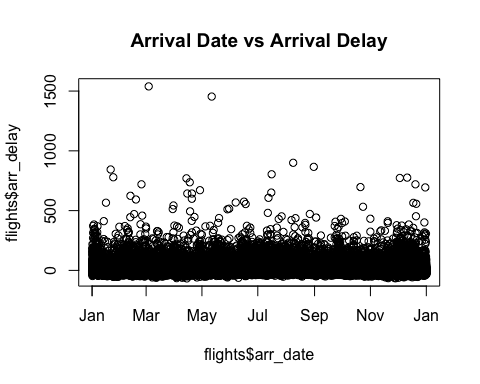
\includegraphics{HW4_files/figure-latex/unnamed-chunk-13-1.pdf}

\begin{Shaded}
\begin{Highlighting}[]
\FunctionTok{plot}\NormalTok{(flights}\SpecialCharTok{$}\NormalTok{dep\_date, flights}\SpecialCharTok{$}\NormalTok{arr\_delay, }\AttributeTok{main =} \StringTok{"Departure Date vs Arrival Delay"}\NormalTok{)}
\end{Highlighting}
\end{Shaded}

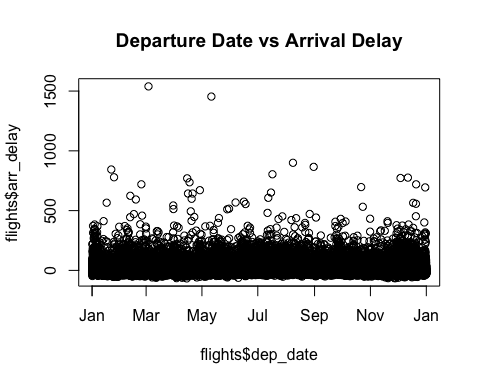
\includegraphics{HW4_files/figure-latex/unnamed-chunk-13-2.pdf}

\begin{Shaded}
\begin{Highlighting}[]
\CommentTok{\#These variables are highly correlated}
\FunctionTok{plot}\NormalTok{(flights}\SpecialCharTok{$}\NormalTok{dep\_delay, flights}\SpecialCharTok{$}\NormalTok{arr\_delay)}
\end{Highlighting}
\end{Shaded}

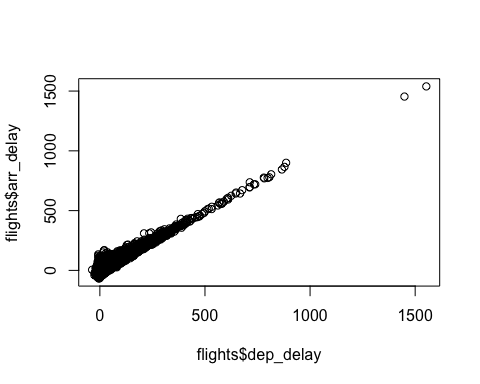
\includegraphics{HW4_files/figure-latex/unnamed-chunk-13-3.pdf}

\begin{Shaded}
\begin{Highlighting}[]
\CommentTok{\#try and look for collinearity}

\NormalTok{flights2 }\OtherTok{\textless{}{-}} \FunctionTok{select}\NormalTok{(flights, dep\_delay, arr\_time, arr\_delay, air\_time, distance)}

\FunctionTok{cor}\NormalTok{(flights2) }
\end{Highlighting}
\end{Shaded}

\begin{verbatim}
##              dep_delay    arr_time   arr_delay     air_time     distance
## dep_delay  1.000000000  0.05626588  0.92351496 -0.008110625 -0.003219088
## arr_time   0.056265885  1.00000000  0.06920322 -0.042684748 -0.048964531
## arr_delay  0.923514961  0.06920322  1.00000000 -0.023384820 -0.054510499
## air_time  -0.008110625 -0.04268475 -0.02338482  1.000000000  0.985321253
## distance  -0.003219088 -0.04896453 -0.05451050  0.985321253  1.000000000
\end{verbatim}

From our correlation matrix, we notice a high degree of correlation
between arr\_delay and dep\_delay, as well as between distance and
air\_time. We will need to keep this in mind when designing our model,
as collinearity violates the assumptions of linear regression.

Now we will remove unnecessary/duplicate features make a simple OLS
model, and then evaluate it's predictive accuracy:

\begin{Shaded}
\begin{Highlighting}[]
\NormalTok{flights2 }\OtherTok{\textless{}{-}} \FunctionTok{select}\NormalTok{(flights, }\SpecialCharTok{{-}}\FunctionTok{c}\NormalTok{(month, day, year, date))}


\NormalTok{flights2}\SpecialCharTok{$}\NormalTok{dep\_date }\OtherTok{\textless{}{-}} \FunctionTok{as.Date}\NormalTok{(flights2}\SpecialCharTok{$}\NormalTok{dep\_date)}

\CommentTok{\#Test/Train Split}
\NormalTok{trainIndex }\OtherTok{\textless{}{-}} \FunctionTok{createDataPartition}\NormalTok{(flights2}\SpecialCharTok{$}\NormalTok{arr\_delay, }\AttributeTok{p =}\NormalTok{ .}\DecValTok{8}\NormalTok{, }
                                  \AttributeTok{list =} \ConstantTok{FALSE}\NormalTok{, }
                                  \AttributeTok{times =} \DecValTok{1}\NormalTok{)}
\NormalTok{train }\OtherTok{\textless{}{-}}\NormalTok{ flights2[trainIndex,]}
\NormalTok{test }\OtherTok{\textless{}{-}}\NormalTok{ flights2[}\SpecialCharTok{{-}}\NormalTok{trainIndex,]}
\end{Highlighting}
\end{Shaded}

\begin{Shaded}
\begin{Highlighting}[]
\CommentTok{\#simple regressions}
\NormalTok{simple1 }\OtherTok{\textless{}{-}} \FunctionTok{lm}\NormalTok{(arr\_delay }\SpecialCharTok{\textasciitilde{}}\NormalTok{ air\_time, }\AttributeTok{data =}\NormalTok{ train)}
\NormalTok{simple1\_predict }\OtherTok{\textless{}{-}} \FunctionTok{predict}\NormalTok{(simple1, test)}
\FunctionTok{RMSE}\NormalTok{(simple1\_predict, test}\SpecialCharTok{$}\NormalTok{arr\_delay)}
\end{Highlighting}
\end{Shaded}

\begin{verbatim}
## [1] 30.86496
\end{verbatim}

RMSE = 31.3

\begin{Shaded}
\begin{Highlighting}[]
\NormalTok{simple2 }\OtherTok{\textless{}{-}} \FunctionTok{lm}\NormalTok{(arr\_delay }\SpecialCharTok{\textasciitilde{}}\NormalTok{ air\_time}\SpecialCharTok{+}\NormalTok{carrier}\SpecialCharTok{+}\NormalTok{origin}\SpecialCharTok{+}\NormalTok{distance}\SpecialCharTok{+}\NormalTok{dest}\SpecialCharTok{+}\NormalTok{dep\_date, }\AttributeTok{data =}\NormalTok{ train)}
\NormalTok{simple2\_predict }\OtherTok{\textless{}{-}} \FunctionTok{predict}\NormalTok{(simple2, test)}
\FunctionTok{RMSE}\NormalTok{(simple2\_predict, test}\SpecialCharTok{$}\NormalTok{arr\_delay)}
\end{Highlighting}
\end{Shaded}

\begin{verbatim}
## [1] 29.58655
\end{verbatim}

RMSE = 30.28

\begin{Shaded}
\begin{Highlighting}[]
\CommentTok{\# Define training control}
\FunctionTok{set.seed}\NormalTok{(}\DecValTok{123}\NormalTok{) }
\NormalTok{train.control }\OtherTok{\textless{}{-}} \FunctionTok{trainControl}\NormalTok{(}\AttributeTok{method =} \StringTok{"cv"}\NormalTok{, }\AttributeTok{number =} \DecValTok{10}\NormalTok{)}

\CommentTok{\# Train the model}
\NormalTok{model }\OtherTok{\textless{}{-}} \FunctionTok{train}\NormalTok{(arr\_delay }\SpecialCharTok{\textasciitilde{}}\NormalTok{ air\_time}\SpecialCharTok{+}\NormalTok{carrier}\SpecialCharTok{+}\NormalTok{origin}\SpecialCharTok{+}\NormalTok{distance}\SpecialCharTok{+}\NormalTok{dest}\SpecialCharTok{+}\NormalTok{dep\_date,}\AttributeTok{data =}\NormalTok{ flights2, }\AttributeTok{method =} \StringTok{"lm"}\NormalTok{,}\AttributeTok{trControl =}\NormalTok{ train.control)}

\CommentTok{\#RMSE = 29.88867}
\FunctionTok{print}\NormalTok{(model)}
\end{Highlighting}
\end{Shaded}

\begin{verbatim}
## Linear Regression 
## 
## 145459 samples
##      6 predictor
## 
## No pre-processing
## Resampling: Cross-Validated (10 fold) 
## Summary of sample sizes: 130913, 130914, 130913, 130914, 130912, 130912, ... 
## Resampling results:
## 
##   RMSE      Rsquared    MAE     
##   29.88867  0.08199325  15.34389
## 
## Tuning parameter 'intercept' was held constant at a value of TRUE
\end{verbatim}

\begin{Shaded}
\begin{Highlighting}[]
\NormalTok{simple1 }\OtherTok{\textless{}{-}} \FunctionTok{lm}\NormalTok{(arr\_delay }\SpecialCharTok{\textasciitilde{}}\NormalTok{ air\_time, }\AttributeTok{data =}\NormalTok{ flights2)}
\NormalTok{simple2 }\OtherTok{\textless{}{-}} \FunctionTok{lm}\NormalTok{(arr\_delay }\SpecialCharTok{\textasciitilde{}}\NormalTok{ air\_time}\SpecialCharTok{+}\NormalTok{carrier}\SpecialCharTok{+}\NormalTok{origin}\SpecialCharTok{+}\NormalTok{distance}\SpecialCharTok{+}\NormalTok{dest}\SpecialCharTok{+}\NormalTok{dep\_date, }\AttributeTok{data =}\NormalTok{ flights2)}
\NormalTok{simple3 }\OtherTok{\textless{}{-}} \FunctionTok{lm}\NormalTok{(arr\_delay }\SpecialCharTok{\textasciitilde{}}\NormalTok{ origin}\SpecialCharTok{+}\NormalTok{dest}\SpecialCharTok{+}\NormalTok{carrier}\SpecialCharTok{+}\NormalTok{distance}\SpecialCharTok{+}\NormalTok{dep\_delay, }\AttributeTok{data =}\NormalTok{ flights2)}
\NormalTok{simple4 }\OtherTok{\textless{}{-}} \FunctionTok{lm}\NormalTok{(arr\_delay }\SpecialCharTok{\textasciitilde{}}\NormalTok{ origin}\SpecialCharTok{+}\NormalTok{dest}\SpecialCharTok{+}\NormalTok{carrier}\SpecialCharTok{+}\NormalTok{distance}\SpecialCharTok{+}\NormalTok{dep\_delay}\SpecialCharTok{+}\NormalTok{dep\_date, }\AttributeTok{data =}\NormalTok{ flights2)}
\NormalTok{simple5 }\OtherTok{\textless{}{-}} \FunctionTok{lm}\NormalTok{(arr\_delay }\SpecialCharTok{\textasciitilde{}}\NormalTok{ origin}\SpecialCharTok{+}\NormalTok{carrier}\SpecialCharTok{+}\NormalTok{distance}\SpecialCharTok{+}\NormalTok{dep\_delay}\SpecialCharTok{+}\NormalTok{dep\_date, }\AttributeTok{data =}\NormalTok{ flights2)}


\FunctionTok{summary}\NormalTok{(simple1)}
\FunctionTok{summary}\NormalTok{(simple2)}
\FunctionTok{summary}\NormalTok{(simple3)}
\end{Highlighting}
\end{Shaded}

\begin{Shaded}
\begin{Highlighting}[]
\NormalTok{simple2\_predict }\OtherTok{\textless{}{-}} \FunctionTok{predict}\NormalTok{(simple2, test)}
\FunctionTok{RMSE}\NormalTok{(simple2\_predict, test}\SpecialCharTok{$}\NormalTok{arr\_delay)}
\end{Highlighting}
\end{Shaded}

\begin{verbatim}
## [1] 29.58655
\end{verbatim}

\begin{Shaded}
\begin{Highlighting}[]
\FunctionTok{summary}\NormalTok{(simple2)}
\end{Highlighting}
\end{Shaded}

\begin{verbatim}
## 
## Call:
## lm(formula = arr_delay ~ air_time + carrier + origin + distance + 
##     dest + dep_date, data = train)
## 
## Residuals:
##     Min      1Q  Median      3Q     Max 
##  -56.54  -12.99   -6.01    2.92 1544.52 
## 
## Coefficients:
##               Estimate Std. Error t value Pr(>|t|)    
## (Intercept) -2.136e+01  1.473e+01  -1.450 0.147127    
## air_time     8.201e-01  9.459e-03  86.701  < 2e-16 ***
## carrierAS   -2.808e+00  6.770e-01  -4.148 3.36e-05 ***
## carrierB6    9.195e+00  1.050e+00   8.756  < 2e-16 ***
## carrierDL    1.972e+00  8.056e-01   2.447 0.014389 *  
## carrierF9    6.254e+00  1.046e+00   5.978 2.26e-09 ***
## carrierHA    6.025e+00  1.440e+00   4.184 2.87e-05 ***
## carrierOO    6.244e-01  7.752e-01   0.806 0.420530    
## carrierUA   -3.043e+00  7.111e-01  -4.280 1.87e-05 ***
## carrierUS   -3.812e+00  9.943e-01  -3.834 0.000126 ***
## carrierVX   -5.317e+00  9.394e-01  -5.660 1.52e-08 ***
## carrierWN    4.510e+00  7.555e-01   5.970 2.38e-09 ***
## originSEA    3.766e+00  2.936e-01  12.825  < 2e-16 ***
## distance    -1.098e-01  3.400e-03 -32.299  < 2e-16 ***
## destANC     -9.575e+00  1.564e+00  -6.122 9.30e-10 ***
## destATL      2.315e+01  3.520e+00   6.576 4.84e-11 ***
## destAUS      1.141e+01  2.788e+00   4.093 4.25e-05 ***
## destBLI     -1.268e+01  5.136e+00  -2.468 0.013572 *  
## destBNA      8.533e+00  4.001e+00   2.133 0.032963 *  
## destBOI     -1.526e+01  4.448e+00  -3.431 0.000601 ***
## destBOS      2.649e+01  4.519e+00   5.861 4.61e-09 ***
## destBUR     -8.550e+00  1.677e+00  -5.097 3.45e-07 ***
## destBWI      2.466e+01  4.294e+00   5.742 9.39e-09 ***
## destBZN     -2.010e+01  2.134e+01  -0.942 0.346417    
## destCLE      4.067e+01  5.885e+00   6.911 4.85e-12 ***
## destCLT      2.750e+01  3.951e+00   6.961 3.39e-12 ***
## destCOS     -4.834e-01  2.241e+00  -0.216 0.829248    
## destCVG      1.306e+01  3.967e+00   3.292 0.000994 ***
## destDCA      2.399e+01  4.074e+00   5.888 3.91e-09 ***
## destDEN      5.680e-01  1.343e+00   0.423 0.672435    
## destDFW      1.505e+01  2.081e+00   7.230 4.86e-13 ***
## destDTW      1.773e+01  2.841e+00   6.240 4.39e-10 ***
## destEUG     -1.815e+01  3.744e+00  -4.849 1.24e-06 ***
## destEWR      2.948e+01  4.195e+00   7.028 2.11e-12 ***
## destFAI     -6.742e+00  1.932e+00  -3.489 0.000485 ***
## destFAT     -8.890e+00  2.258e+00  -3.937 8.25e-05 ***
## destFLL      2.858e+01  5.354e+00   5.338 9.42e-08 ***
## destGEG     -1.258e+01  3.411e+00  -3.688 0.000226 ***
## destHDN      6.942e+00  6.885e+00   1.008 0.313377    
## destHNL      7.749e-03  4.970e+00   0.002 0.998756    
## destHOU      1.464e+01  3.610e+00   4.055 5.02e-05 ***
## destIAD      3.044e+01  3.964e+00   7.679 1.61e-14 ***
## destIAH      1.697e+01  2.597e+00   6.536 6.36e-11 ***
## destJAC     -9.528e+00  9.303e+00  -1.024 0.305725    
## destJFK      2.684e+01  4.279e+00   6.273 3.56e-10 ***
## destJNU     -1.147e+01  1.798e+00  -6.381 1.77e-10 ***
## destKOA     -4.836e+00  5.100e+00  -0.948 0.343015    
## destKTN     -1.225e+01  2.256e+00  -5.427 5.73e-08 ***
## destLAS     -9.719e+00  1.627e+00  -5.973 2.33e-09 ***
## destLAX     -7.002e+00  1.490e+00  -4.701 2.60e-06 ***
## destLGB     -1.946e+01  1.674e+00 -11.628  < 2e-16 ***
## destLIH     -4.498e+00  5.176e+00  -0.869 0.384858    
## destLMT     -2.890e+01  4.239e+00  -6.818 9.27e-12 ***
## destMCI      6.923e+00  1.996e+00   3.468 0.000525 ***
## destMCO      2.495e+01  4.811e+00   5.185 2.16e-07 ***
## destMDW      5.040e+00  2.368e+00   2.129 0.033295 *  
## destMIA      3.782e+01  5.449e+00   6.941 3.90e-12 ***
## destMKE      8.799e+00  2.734e+00   3.218 0.001291 ** 
## destMSP      4.871e+00  1.571e+00   3.100 0.001934 ** 
## destMSY      3.176e+00  3.959e+00   0.802 0.422502    
## destOAK     -1.059e+01  2.115e+00  -5.008 5.50e-07 ***
## destOGG     -3.134e+00  4.868e+00  -0.644 0.519688    
## destOMA      5.147e+00  2.309e+00   2.229 0.025845 *  
## destONT     -8.481e+00  1.666e+00  -5.090 3.59e-07 ***
## destORD      2.012e+01  2.227e+00   9.037  < 2e-16 ***
## destPDX     -2.155e+01  3.658e+00  -5.891 3.86e-09 ***
## destPHL      3.049e+01  4.180e+00   7.294 3.03e-13 ***
## destPHX     -2.493e+00  1.303e+00  -1.914 0.055673 .  
## destPSP     -9.039e+00  1.798e+00  -5.028 4.97e-07 ***
## destRDM     -1.727e+01  3.667e+00  -4.708 2.50e-06 ***
## destRNO     -9.335e+00  3.095e+00  -3.016 0.002559 ** 
## destSAN     -7.063e+00  1.382e+00  -5.111 3.20e-07 ***
## destSAT      6.916e+00  2.893e+00   2.391 0.016816 *  
## destSBA     -8.043e+00  2.070e+00  -3.884 0.000103 ***
## destSEA     -1.879e+01  3.471e+00  -5.414 6.17e-08 ***
## destSFO     -7.624e+00  2.135e+00  -3.571 0.000355 ***
## destSIT     -1.095e+01  3.858e+00  -2.839 0.004520 ** 
## destSJC     -1.360e+01  2.063e+00  -6.594 4.29e-11 ***
## destSLC     -9.248e+00  2.054e+00  -4.503 6.70e-06 ***
## destSMF     -6.690e+00  2.298e+00  -2.911 0.003606 ** 
## destSNA     -1.217e+01  1.532e+00  -7.944 1.97e-15 ***
## destSTL      1.312e+01  2.607e+00   5.034 4.80e-07 ***
## destTPA      5.719e+00  5.080e+00   1.126 0.260284    
## destTUS     -3.269e+00  1.786e+00  -1.831 0.067136 .  
## dep_date     1.797e-03  8.752e-04   2.053 0.040096 *  
## ---
## Signif. codes:  0 '***' 0.001 '**' 0.01 '*' 0.05 '.' 0.1 ' ' 1
## 
## Residual standard error: 29.99 on 116284 degrees of freedom
## Multiple R-squared:  0.0824, Adjusted R-squared:  0.08174 
## F-statistic: 124.3 on 84 and 116284 DF,  p-value: < 2.2e-16
\end{verbatim}

\begin{Shaded}
\begin{Highlighting}[]
\FunctionTok{lrtest}\NormalTok{(simple1, simple2)}
\end{Highlighting}
\end{Shaded}

\begin{verbatim}
## Likelihood ratio test
## 
## Model 1: arr_delay ~ air_time
## Model 2: arr_delay ~ air_time + carrier + origin + distance + dest + dep_date
##   #Df  LogLik Df  Chisq Pr(>Chisq)    
## 1   3 -565820                         
## 2  86 -560847 83 9946.9  < 2.2e-16 ***
## ---
## Signif. codes:  0 '***' 0.001 '**' 0.01 '*' 0.05 '.' 0.1 ' ' 1
\end{verbatim}

\begin{Shaded}
\begin{Highlighting}[]
\FunctionTok{plot}\NormalTok{(simple2)}
\end{Highlighting}
\end{Shaded}

\includegraphics{HW4_files/figure-latex/unnamed-chunk-20-1.pdf}
\includegraphics{HW4_files/figure-latex/unnamed-chunk-20-2.pdf}
\includegraphics{HW4_files/figure-latex/unnamed-chunk-20-3.pdf}
\includegraphics{HW4_files/figure-latex/unnamed-chunk-20-4.pdf}

For this problem, I originally thought of using machine learning
methods, as I thought that these would be able to make models with very
high predictive accuracy. Interestingly I noticed that the model that I
settled on had an RMSE of 30.028, whereas my best machine learning model
using a 10 k fold split was only able to achieve an RMSE of 29.8.

This lead me to think about the problem in a new way, as the goal of
this problem is statistical inference, and thus making a model that fits
well is more important than making a model that predicts well. I
eventually decided to use OLS as it would be easy to interpret, and I
used variables that were likely to have an effect on arrival delay. I
avoided using both air\_time and distance, as these variables are highly
correlated, and I did not want to violate the collinearity assumption.

I chose to fit an OLS regression on arr\_delay, with the following
variables as predictors:
origin,dest,carrier,distance,dep\_delay,dep\_date. This model achieved
an R\^{}2 of 0.86, which is much higher than my simplest model's R\^{}2
of 0.081. Relative to my simplest model, we can also confirm using the
likelihood ratio test that my model fits the data better (p \textless{}
0.0001).

From the cook's vs distance plot, we can see that there are very few
influential values, and from the Normal Q-Q plot, we can verify the
normality assumption. Most of the variables in this model were
statistical significant, with the exception of a few carriers and
origin/destination airports.

What this model shows us, is that for this dataset, there exists a
relationship between the predictors and arrival delay, and approximately
87\% of the variability in the data can be explained by the model.

\textbf{Difference in Means Test}

\begin{Shaded}
\begin{Highlighting}[]
\NormalTok{df }\OtherTok{\textless{}{-}} \FunctionTok{subset}\NormalTok{(flights, carrier }\SpecialCharTok{==} \StringTok{"F9"} \SpecialCharTok{|}\NormalTok{ carrier }\SpecialCharTok{==} \StringTok{"US"}\NormalTok{)}

\NormalTok{df }\OtherTok{\textless{}{-}} \FunctionTok{select}\NormalTok{(df, carrier, arr\_delay)}

\FunctionTok{hist}\NormalTok{(df}\SpecialCharTok{$}\NormalTok{arr\_delay[df}\SpecialCharTok{$}\NormalTok{carrier }\SpecialCharTok{==} \StringTok{"F9"}\NormalTok{], }\AttributeTok{main =} \StringTok{"Distribution of F9 Carrier Arrival Delay"}\NormalTok{,}
     \AttributeTok{xlim =} \FunctionTok{range}\NormalTok{(}\DecValTok{0}\SpecialCharTok{:}\DecValTok{200}\NormalTok{), }\AttributeTok{xlab =} \StringTok{"Arrival Delay (minutes)"}\NormalTok{)}
\end{Highlighting}
\end{Shaded}

\includegraphics{HW4_files/figure-latex/unnamed-chunk-21-1.pdf}

\begin{Shaded}
\begin{Highlighting}[]
\FunctionTok{hist}\NormalTok{(df}\SpecialCharTok{$}\NormalTok{arr\_delay[df}\SpecialCharTok{$}\NormalTok{carrier }\SpecialCharTok{==} \StringTok{"US"}\NormalTok{], }\AttributeTok{main =} \StringTok{"Distribution of US Carrier Arrival Delay"}\NormalTok{,}
     \AttributeTok{xlim =} \FunctionTok{range}\NormalTok{(}\DecValTok{0}\SpecialCharTok{:}\DecValTok{200}\NormalTok{), }\AttributeTok{xlab =} \StringTok{"Arrival Delay (minutes)"}\NormalTok{)}
\end{Highlighting}
\end{Shaded}

\includegraphics{HW4_files/figure-latex/unnamed-chunk-21-2.pdf}

The conditions for conducting a difference in means test are that the
samples are obtained randomly. I am not completely sure where this data
came from but I will assume for now that the samples are obtained
randomly.

Since each row represents a different flight, it is fair to assume that
samples are independent, and that one flight does not affect another. In
any case where it would like a certain accident on the runway causing
delays of other flights, this variability will be mitigated by random
sampling.

The histograms above do not appear to depict the sampling distribution
as normal. However, since the sample size is greater than 40 for both
airlines, we can meet the normality assumption.

\begin{Shaded}
\begin{Highlighting}[]
\FunctionTok{t.test}\NormalTok{(arr\_delay }\SpecialCharTok{\textasciitilde{}}\NormalTok{ carrier, }\AttributeTok{data =}\NormalTok{ df)}
\end{Highlighting}
\end{Shaded}

\begin{verbatim}
## 
##  Welch Two Sample t-test
## 
## data:  arr_delay by carrier
## t = 11.405, df = 3405.8, p-value < 2.2e-16
## alternative hypothesis: true difference in means between group F9 and group US is not equal to 0
## 95 percent confidence interval:
##   8.730665 12.355621
## sample estimates:
## mean in group F9 mean in group US 
##         9.201161        -1.341982
\end{verbatim}

Our t test returned a p value of \textless{} 2.2e-16 for the null
hypothesis that the true difference in means is equal to zero. Sample
sizes were significantly large with 2411 F9 flights and 5319 US flights.
This means that we can reject the null hypothesis, and confirm that the
true difference in means is not zero. A 95\% confidence interval for the
true difference in means was {[}8.730665, 12.355621{]} and zero is
notably not in the confidence interval.

\textbf{Conclusion}

Our regression model provided a coefficient of 5.669208 for having F9 as
carrier and a coefficient of -4.472456 for having US as a carrier, and
both coefficients were statistically. Our difference in means test
showed that there is definitely a difference in the mean flight time
between F9 and US. If trying to make a decision solely based on airline,
the professor should definitely pick US airlines, as they are
statistically likely to be early compared to other airlines.

However the following histogram shows the distribution of all of the
regression coefficients:

\begin{Shaded}
\begin{Highlighting}[]
\FunctionTok{hist}\NormalTok{(}\FunctionTok{coef}\NormalTok{(simple2), }\AttributeTok{xlab =} \StringTok{"coefficient value"}\NormalTok{, }\AttributeTok{main =} \StringTok{"Distribution of Regression coefficients"}\NormalTok{)}
\end{Highlighting}
\end{Shaded}

\includegraphics{HW4_files/figure-latex/unnamed-chunk-23-1.pdf}

From observing the distribution, we observe that 5.6 and -4.4 appear to
be relatively in the center, meaning that they do not have as big of an
effect on arrival time as other variables in the model. While it is
likely to be the case that picking US airlines would decrease the flight
time, other variables are likely to have a higher chance at decreasing
flight time. For example, having Cleavland as a destination has a
coefficient of 40, and is much more likely to increase flight time.
Additionally, having LMT as a destination has a coefficient of -28 and
is much more likely to decrease flight time.

\end{document}
